\documentclass[handout]{beamer}\usepackage[]{graphicx}\usepackage[]{color}
%% maxwidth is the original width if it is less than linewidth
%% otherwise use linewidth (to make sure the graphics do not exceed the margin)
\makeatletter
\def\maxwidth{ %
  \ifdim\Gin@nat@width>\linewidth
    \linewidth
  \else
    \Gin@nat@width
  \fi
}
\makeatother

\definecolor{fgcolor}{rgb}{0.345, 0.345, 0.345}
\newcommand{\hlnum}[1]{\textcolor[rgb]{0.686,0.059,0.569}{#1}}%
\newcommand{\hlstr}[1]{\textcolor[rgb]{0.192,0.494,0.8}{#1}}%
\newcommand{\hlcom}[1]{\textcolor[rgb]{0.678,0.584,0.686}{\textit{#1}}}%
\newcommand{\hlopt}[1]{\textcolor[rgb]{0,0,0}{#1}}%
\newcommand{\hlstd}[1]{\textcolor[rgb]{0.345,0.345,0.345}{#1}}%
\newcommand{\hlkwa}[1]{\textcolor[rgb]{0.161,0.373,0.58}{\textbf{#1}}}%
\newcommand{\hlkwb}[1]{\textcolor[rgb]{0.69,0.353,0.396}{#1}}%
\newcommand{\hlkwc}[1]{\textcolor[rgb]{0.333,0.667,0.333}{#1}}%
\newcommand{\hlkwd}[1]{\textcolor[rgb]{0.737,0.353,0.396}{\textbf{#1}}}%
\let\hlipl\hlkwb

\usepackage{framed}
\makeatletter
\newenvironment{kframe}{%
 \def\at@end@of@kframe{}%
 \ifinner\ifhmode%
  \def\at@end@of@kframe{\end{minipage}}%
  \begin{minipage}{\columnwidth}%
 \fi\fi%
 \def\FrameCommand##1{\hskip\@totalleftmargin \hskip-\fboxsep
 \colorbox{shadecolor}{##1}\hskip-\fboxsep
     % There is no \\@totalrightmargin, so:
     \hskip-\linewidth \hskip-\@totalleftmargin \hskip\columnwidth}%
 \MakeFramed {\advance\hsize-\width
   \@totalleftmargin\z@ \linewidth\hsize
   \@setminipage}}%
 {\par\unskip\endMakeFramed%
 \at@end@of@kframe}
\makeatother

\definecolor{shadecolor}{rgb}{.97, .97, .97}
\definecolor{messagecolor}{rgb}{0, 0, 0}
\definecolor{warningcolor}{rgb}{1, 0, 1}
\definecolor{errorcolor}{rgb}{1, 0, 0}
\newenvironment{knitrout}{}{} % an empty environment to be redefined in TeX

\usepackage{alltt}
%\usepackage[dvips]{color}

\usepackage{graphicx}
\usepackage{amsmath,amssymb,array,eucal}
\usepackage{xcolor}
\definecolor{beamer@blendedblue}{RGB}{86,155,189}
\definecolor{myblue}{RGB}{12,76,138}
\setbeamercolor{structure}{fg=myblue}
\definecolor{Ftitle}{RGB}{12,76,138}
\definecolor{Descitem}{RGB}{238,238,244}
\definecolor{StdTitle}{RGB}{12,76,138}
\definecolor{StdBody}{RGB}{213,24,0}
\definecolor{StdBody}{RGB}{213,24,0}

\definecolor{AlTitle}{RGB}{255, 190, 190}
\definecolor{AlBody}{RGB}{213,24,0}

\definecolor{ExTitle}{RGB}{201, 217, 217}
\definecolor{ExBody}{RGB}{213,24,0}

\setbeamercolor{frametitle}{fg = Ftitle}
\setbeamercolor{title}{fg = Ftitle}
\setbeamercolor{item}{fg = Ftitle}
\setbeamercolor{subitem}{fg = Ftitle}
\setbeamercolor{subsubitem}{fg = Ftitle}
\setbeamercolor{description item}{fg = myblue}
\setbeamercolor{titlelike}{fg=myblue}

%$Id: macros.tex,v 1.2 2006/02/13 14:23:55 rlw Exp rlw $
\newcommand{\Lmea}{{\cal L}} 
\newcommand{\scale}{\bflambda} 
\newcommand{\Scale}{\bfLambda} 
\newcommand{\bfscale}{\bflambda} 
\newcommand{\mean}{\bfchi}
\newcommand{\loc}{\bfchi}
\newcommand{\bfmean}{\bfchi}
\renewcommand{\k}{g}
\newcommand{\Gen}{{\cal G}}
\newcommand{\eps}{\epsilon}

\newcommand{\ind}{\mathrel{\mathop{\sim}\limits^{\mathit{ind}}}}
\newcommand{\iid}{\mathrel{\mathop{\sim}\limits^{\mathit{iid}}}}
\newcommand{\dis}{\mathrel{\mathop{=}\limits^{d}}}
\newcommand{\sgn}{\mathop{\rm sgn}}
\newcommand{\cmp}{h}
\newcommand{\dbdo}{d\beta ~ d\omega}
\newcommand{\real}{{\mathbb{R}}}
\newcommand{\Ber}{\mbox{\rm Ber}}
\newcommand{\GP}{\mbox{\rm GP}}
\newcommand{\SaS}{\text{S$\alpha$S}}
\newcommand{\RA}{{\real \times A}}
\newcommand{\RK}{{\real \times K}}
\newcommand{\RO}{{\real \times \Omega}} 
\newcommand{\RS}{{\bbR \times \LamS}}
  \newcommand{\set}[1]{\left\{#1\right\}}
  \newcommand{\bet}[1]{\left[#1\right]}
  \newcommand{\cet}[1]{\left(#1\right)}
%  \renewcommand{\half}{{\scriptstyle\frac12}}
\newcommand{\subA}{(\eps_1 < \beta \le \eps_2) \times \LamS}
 \newcommand{\uu}{{\big(\scale(x - \loc)\big)}}
 \newcommand{\uuj}{{\big(\scale_j(x-\loc_j)\big)}}
 \newcommand{\bbT}{{\mathbb{T}}}
 \newcommand{\ui}{{[0,1)}}
 \newcommand{\spq}[1]{\left|#1\right|^s_{pq}}
 \newcommand{\spqper}[1]{\left|#1\right|^{s\,*}_{pq}}
 \newcommand{\sspqper}[1]{\left\|#1\right\|^{s\,*}_{pq}}
 \newcommand{\sspq}[1]{\left\|#1\right\|^s_{pq}}    % Besov semi-norm
 \newcommand{\qp}[1]  {\left\|#1\right\|^q_p}         % Hilbert-space norm
 \newcommand{\qper}[1]{\left\|#1\right\|^{*\,q}_p}  % Periodic HS norm
 

\newcommand{\bbW}{{\mathbb{W}}}
\newcommand{\bbB}{{\mathbb{B}}}
\newcommand{\Sob}{{\ensuremath{\bbW^s_2}}}
\newcommand{\Besov}{{\ensuremath{\bbB^s_{pq}}}}
\newcommand{\Besper}{{\ensuremath{\bbB^{s\,*}_{pq}}}}
\newcommand{\Sobx}[1]{{\bbW^{#1}_2}}
\newcommand{\Besovx}[1]{{\bbB^{#1}_2}}
\newcommand{\SN}[1]{\|{#1}\|_\Sob}
% MATH LETTER DEFINITIONS
\newcommand{\Levy}{L{\'e}vy}
\newcommand{\nmathbf}{\bm}
\newcommand{\tabb}[1]{\hspace*{#1\parindent}}
%\newcommand{\G}{{g}}    % Really the same as \GB
\newcommand{\g}{{\phi}} %\newcommand{\g}{{g}}
\newcommand{\GB}{{g}}  
% Roman math Bold face 


\def\bfA{\nmathbf A}
\def\bfB{\nmathbf B}
\def\bfC{\nmathbf C}
\def\bfD{\nmathbf D}
\def\bfE{\nmathbf E}
\def\bfF{\nmathbf F}
\def\bfG{\nmathbf G}
\def\bfH{\nmathbf H}
\def\bfI{\nmathbf I}
\def\bfJ{\nmathbf J}
\def\bfK{\nmathbf K}
\def\bfL{\nmathbf L}
\def\bfM{\nmathbf M}
\def\bfN{\nmathbf N}
\def\bfO{\nmathbf O}
\def\bfP{\nmathbf P}
\def\bfQ{\nmathbf Q}
\def\bfR{\nmathbf R}
\def\bfS{\nmathbf S}
\def\bfT{\nmathbf T}
\def\bfU{\nmathbf U}
\def\bfV{\nmathbf V}
\def\bfW{\nmathbf W}
\def\bfX{\nmathbf X}
\def\bfY{\nmathbf Y}
\def\bfZ{\nmathbf Z}

\def\bfa{\nmathbf a}
\def\bfb{\nmathbf b}
\def\bfc{\nmathbf c}
\def\bfd{\nmathbf d}
\def\bfe{\nmathbf e}
\def\bff{\nmathbf f}
\def\bfg{\nmathbf g}
\def\bfh{\nmathbf h}
\def\bfi{\nmathbf i}
\def\bfj{\nmathbf j}
\def\bfk{\nmathbf k}
\def\bfl{\nmathbf l}
\def\bfm{\nmathbf m}
\def\bfn{\nmathbf n}
\def\bfo{\nmathbf o}
\def\bfp{\nmathbf p}
\def\bfq{\nmathbf q}
\def\bfr{\nmathbf r}
\def\bfs{\nmathbf s}
\def\bft{\nmathbf t}
\def\bfu{\nmathbf u}
\def\bfv{\nmathbf v}
\def\bfw{\nmathbf w}
\def\bfx{\nmathbf x}
\def\bfy{\nmathbf y}
\def\bfz{\nmathbf z}


\def\bfalpha  {\nmathbf \alpha}
\def\bfbeta   {\nmathbf \beta}
\def\bfgamma  {\nmathbf \gamma}
\def\bfdelta  {\nmathbf \delta}
\def\bfepsilon{\nmathbf \epsilon}
\def\bfvareps {\nmathbf \varepsilon}
\def\bfzeta   {\nmathbf \zeta}
\def\bfeta    {\nmathbf \eta}
\def\bftheta  {\nmathbf \theta}
\def\bfiota   {\nmathbf \iota}
\def\bfkappa  {\nmathbf \kappa}
\def\bflambda {\nmathbf \lambda}
\def\bfmu     {\nmathbf \mu}
\def\bfnu     {\nmathbf \nu}
\def\bfxi     {\nmathbf \xi}
\def\bfomicron{\nmathbf \omicron}
\def\bfpi     {\nmathbf \pi}
\def\bfrho    {\nmathbf \rho}
\def\bfsigma  {\nmathbf \sigma}
\def\bftau    {\nmathbf \tau}
\def\bfupsilon{\nmathbf \upsilon}
\def\bfphi    {\nmathbf \phi}
\def\bfpsi    {\nmathbf \psi}
\def\bfchi    {\nmathbf \chi}
\def\bfomega  {\nmathbf \omega}
\newcommand{\nubw}{{\tilde\nu}}  % no longer red!
\def\bfAlpha  {\nmathbf \Alpha}
\def\bfBeta   {\nmathbf \Beta}
\def\bfGamma  {\nmathbf \Gamma}
\def\bfDelta  {\nmathbf \Delta}
\def\bfEpsilon{\nmathbf \Epsilon}
\def\bfZeta   {\nmathbf \Zeta}
\def\bfEta    {\nmathbf \Eta}
\def\bfTheta  {\nmathbf \Theta}
\def\bfIota   {\nmathbf \Iota}
\def\bfKappa  {\nmathbf \Kappa}
\def\bfLambda {\nmathbf \Lambda}
\def\bfMu     {\nmathbf \Mu}
\def\bfNu     {\nmathbf \Nu}
\def\bfXi     {\nmathbf \Xi}
\def\bfOmicron{\nmathbf \Omicron}
\def\bfPi     {\nmathbf \Pi}
\def\bfRho    {\nmathbf \Rho}
\def\bfSigma  {\nmathbf \Sigma}
\def\bfTau    {\nmathbf \Tau}
\def\bfUpsilon{\nmathbf \Upsilon}
\def\bfPhi    {\nmathbf \Phi}
\def\bfPsi    {\nmathbf \Psi}
\def\bfChi    {\nmathbf \Chi}
\def\bfOmega  {\nmathbf \Omega}

% Number math Bold face

\newcommand{\bfzero}{{\nmathbf 0}}
\newcommand{\bfone}{{\nmathbf 1}}

% Estimators

\newcommand{\ttheta}{\tilde{\theta}}
\newcommand{\htheta}{\hat{\theta}}
\newcommand{\tbtheta}{\tilde{\bftheta}}
\newcommand{\hbtheta}{\hat{\bftheta}}
\newcommand{\tomega}{\tilde{\omega}}
\newcommand{\homega}{\hat{\omega}}
\newcommand{\tbomega}{\tilde{\bfomega}}
\newcommand{\hbomega}{\hat{\bfomega}}
\newcommand{\tlambda}{\tilde{\lambda}}
\newcommand{\hlambda}{\hat{\lambda}}
\newcommand{\tblambda}{\tilde{\bflambda}}
\newcommand{\hblambda}{\hat{\bflambda}}


% Calligraphic

\newcommand{\mc}[1]{\ensuremath{\mathcal{#1}}}

\newcommand{\cfA}{\mc{A}}
\newcommand{\cfB}{\mc{B}}
\newcommand{\cfC}{\mc{C}}
\newcommand{\cfD}{\mc{D}}
\newcommand{\cfE}{\mc{E}}
\newcommand{\cfF}{\mc{F}}
\newcommand{\cfG}{\mc{G}}
\newcommand{\cfH}{\mc{H}}
\newcommand{\cfI}{\mc{I}}
\newcommand{\cfJ}{\mc{J}}
\newcommand{\cfK}{\mc{K}}
\newcommand{\cfL}{\mc{L}}
\newcommand{\cfM}{\mc{M}}
\newcommand{\cfN}{\mc{N}}
\newcommand{\cfO}{\mc{O}}
\newcommand{\cfP}{\mc{P}}
\newcommand{\cfQ}{\mc{Q}}
\newcommand{\cfR}{\mc{R}}
\newcommand{\cfS}{\mc{S}}
\newcommand{\cfT}{\mc{T}}
\newcommand{\cfU}{\mc{U}}
\newcommand{\cfV}{\mc{V}}
\newcommand{\cfX}{\mc{X}}
\newcommand{\cfY}{\mc{Y}}
\newcommand{\cfZ}{\mc{Z}}

\newcommand{\bmc}[1]{\ensuremath{\boldsymbol{\mathcal{#1}}}}

\newcommand{\bcfA}{\bmc{A}}
\newcommand{\bcfB}{\bmc{B}}
\newcommand{\bcfC}{\bmc{C}}
\newcommand{\bcfD}{\bmc{D}}
\newcommand{\bcfE}{\bmc{E}}
\newcommand{\bcfF}{\bmc{F}}
\newcommand{\bcfG}{\bmc{G}}
\newcommand{\bcfH}{\bmc{H}}
\newcommand{\bcfI}{\bmc{I}}
\newcommand{\bcfJ}{\bmc{J}}
\newcommand{\bcfK}{\bmc{K}}
\newcommand{\bcfL}{\bmc{L}}
\newcommand{\bcfM}{\bmc{M}}
\newcommand{\bcfN}{\bmc{N}}
\newcommand{\bcfO}{\bmc{O}}
\newcommand{\bcfP}{\bmc{P}}
\newcommand{\bcfQ}{\bmc{Q}}
\newcommand{\bcfR}{\bmc{R}}
\newcommand{\bcfS}{\bmc{S}}
\newcommand{\bcfT}{\bmc{T}}
\newcommand{\bcfU}{\bmc{U}}
\newcommand{\bcfV}{\bmc{V}}
\newcommand{\bcfW}{\bmc{W}}
\newcommand{\bcfX}{\bmc{X}}
\newcommand{\bcfY}{\bmc{Y}}
\newcommand{\bcfZ}{\bmc{Z}}

% Special symbols

\newcommand{\reals}{\mbox{\rm I\kern-.20em R}}
\newcommand{\sreals}{\mbox{\small \rm I\kern-.20em R}}
\newcommand{\LamS}{{\cS^d_+}}

% MATHEMATICAL NOTATION

% Operators

\newcommand{\bg}{\;\bigg\vert\;}
\newcommand{\pr}{\mbox{\rm Pr}}
\newcommand{\D}{\mbox{\rm D}}
\newcommand{\E}{\mbox{\rm E}}
\newcommand{\Mo}{\mbox{\rm Mo}}
\newcommand{\Me}{\mbox{\rm Me}}
\newcommand{\Cov}{\mbox{\rm Cov}}
\newcommand{\Var}{\mbox{\rm Var}}
\newcommand{\Corr}{\mbox{\rm Corr}}
\newcommand{\Q}{\mbox{\rm Q}}

% Distributions
\newcommand{\BeBi}{\mbox{\rm BeBi}}
\newcommand{\Be}{\mbox{\rm Be}}
\newcommand{\Bi}{\mbox{\rm Bi}}
\newcommand{\Br}{\mbox{\rm Br}}
\newcommand{\Ca}{\mbox{\rm Ca}}
\newcommand{\Di}{\mbox{\rm Di}}
\newcommand{\Ex}{\mbox{\rm Ex}}
\newcommand{\Fs}{\mbox{\rm Fs}}
\newcommand{\Ga}{\mbox{\sf G}}
\newcommand{\Ge}{\mbox{\rm Ge}}
\newcommand{\GaGa}{\mbox{\rm GaGa}}
\newcommand{\Hy}{\mbox{\rm Hy}}
\newcommand{\IGa}{\mbox{\rm IGa}}
\newcommand{\IPa}{\mbox{\rm IPa}}
\newcommand{\Lo}{\mbox{\rm Lo}}
\newcommand{\Mu}{\mbox{\rm Mu}}
\newcommand{\N}{\mbox{\rm N}}
\newcommand{\NBi}{\mbox{\rm NBi}}
\newcommand{\NGa}{\mbox{\rm NGa}}
\newcommand{\NWi}{\mbox{\rm NWi}}
\newcommand{\Pa}{\mbox{\rm Pa}}
\newcommand{\Po}{\mbox{\sf P}}
\newcommand{\PoGa}{\mbox{\rm PoGa}}
\newcommand{\Ra}{\mbox{\rm Ra}}
\newcommand{\REx}{\mbox{\rm REx}}
\newcommand{\St}{\mbox{\rm St}}
\newcommand{\Un}{\mbox{\rm Un}}
\newcommand{\Wi}{\mbox{\rm Wi}}

% General Mathematics

\newcommand{\dd}[1]{\,d{#1}}
\newcommand{\barx}{\ensuremath{\bar{x}}}
\newcommand{\comb}[2]{{#1\choose#2}}
\newcommand{\ontop}[2]{{#1\atop#2}}
\newcommand{\h}{{\small\ensuremath{1\over2}}}
\newcommand{\hh}[2]{{\small\ensuremath{#1\over#2}}}

\newcommand{\fn}[1]{\hbox{\textrm{#1}}}
\newcommand{\cred}{\fn{Cr}}
\newcommand\dlim{\mathop{\rm \hbox{$\delta$}lim}}
\newcommand{\goto}{\rightarrow}
\newcommand{\gotoinf}{\rightarrow \infty}

\newcommand{\data}{\ensuremath{\bfx=\{x_1,\ldots,x_n\}}}
\newcommand{\brow}[2]{\ensuremath{\{{#1}_1,\ldots,{#1}_{#2}\}}}
\newcommand{\prow}[2]{\ensuremath{({#1}_1,\ldots,{#1}_{#2})}}

\newcommand{\met}{\thinspace{\rm m}}\newcommand{\km}{\thinspace{\rm km}}
\newcommand{\xbar}{\overline X}%
\newcommand{\xbbar}{\overline{\overline X}}%
\font\ss=cmss12
 \newcommand{\OFP}{(\Omega,\cF,\P)}
 \newcommand{\bbC}{\mathbb{C}}
 \newcommand{\bbF}{\mathbb{F}}
 \newcommand{\bbN}{\mathbb{N}}
 \newcommand{\bbR}{\mathbb{R}}
 \newcommand{\bbX}{\mathbb{X}}
 \newcommand{\bbZ}{\mathbb{Z}}
 \newcommand{\one}[1]{\mathbf{1}_{\{#1\}}}
 \newcommand{\cA}{{\cal A}}
 \newcommand{\cB}{{\cal B}} 
 \newcommand{\cE}{{\cal E}}
 \newcommand{\cF}{{\cal F}}
 \newcommand{\cG}{{\cal G}}
 \newcommand{\cH}{{\cal H}}
 \newcommand{\cM}{{\cal M}}
 \newcommand{\cR}{{\cal R}}
 \newcommand{\cS}{{\cal S}}
 \newcommand{\cT}{{\cal T}}
 \newcommand{\cX}{{\cal X}}
 \newcommand{\cY}{{\cal Y}}
 \newcommand{\cZ}{{\cal Z}}
 \newcommand{\eF}{{\CMcal F}}
 \newcommand{\eG}{{\CMcal G}} 
 \newcommand{\eH}{{\CMcal H}}
 \renewcommand{\P}{{\sf{P}}} 
 \renewcommand{\E}{{\sf{E}}}
 \newcommand{\Ev}{{\sf{Ev}}}%
 \newcommand{\V}{{\sf{V}}} 
 \renewcommand{\Cov}{{\sf{Cov}}}
 %\newcommand{\Be}{\textsf{Be}}
 %\newcommand{\Bi}{\textsf{Bi}}
 %\newcommand{\Ex}{\textsf{Ex}}\newcommand{\Ga}{\textsf{Ga}}
 %\newcommand{\Di}{\textsf{Di}}\newcommand{\Ge}{\textsf{Ge}}
 %\newcommand{\IG}{\textsf{IG}}\newcommand{\Lv}{\textsf{Lv}}
 %\newcommand{\HG}{\textsf{HG}}\newcommand{\MN}{\textsf{MN}}
\newcommand{\NB}{\textsf{NB}}\newcommand{\No}{\textsf{N}}
\newcommand{\LN}{\textsf{LN}}
\newcommand{\Lv}{\mbox{\rm Lv}}
%\newcommand{\Pa}{\textsf{Pa}}
% \newcommand{\Po}{\textsf{Po}}\newcommand{\Un}{\textsf{Un}}
 \newcommand{\argmax}{\textrm{argmax}}
 \renewcommand{\th}{{\ensuremath^{\mbox{\tiny th}}}}
 \newcommand{\nd}{{\ensuremath^{\mbox{\tiny nd}}}}
 \newcommand{\st}{{\ensuremath^{\mbox{\tiny st}}}}
 \newcommand{\ii}{{\ensuremath{\bar{i}}}}% \newcommand{\ii}{{\hat i}}
 \newcommand{\jj}{{\ensuremath{\bar{j}}}}%
 \newcommand{\R}{\texttt{R}}
 \newcommand{\mayeq}{\mathrel{\mathop{=}\limits^?}}
 \newcommand{\pperp}{\mathrel{{\rlap{$~\perp$}\perp\,\,}}}
 \newbox\asbox
 \setbox\asbox=\hbox{\vrule height 15pt depth3.5pt width0pt}
 \def\astrut{\relax\ifmmode\copy\strutbox\else\unhcopy\strutbox\fi}
 \def\Strut{\vrule width0pt height 16pt depth 4pt}%
%\font\tinyss=cmss8 at 8truept % for ^T etc
\newcommand{\tsf}[1]{\textsf{\tiny{#1}}}
\newcommand{\fxa}{\mbox{$f(x\mid\alpha)$}}
\newcommand{\fxt}{\mbox{$f(x\mid\theta)$}}
\newcommand{\fxat}{\mbox{$f(x\mid\alpha,\theta)$}}
\newcommand{\tp}{^{\tsf{T}}}
\newcommand{\as}{\textit{a.s.}}
\newcommand{\ie}{\textit{i.e.{}}}
\newcommand{\etc}{\textit{etc}}
\newcommand{\eg}{\textit{e.g.{}}}%
\newcommand{\half}{{\frac12}}
\newcommand{\Sec}[1]{Section\thinspace(\ref{#1})}
\newcommand{\Thm}[1]{Theorem\thinspace\ref{#1}}
\newcommand{\Cor}[1]{Corollary\thinspace\ref{#1}}
\newcommand{\Eqn}[1]{Equation\thinspace(\ref{#1})}
\newcommand{\Fig}[1]{Figure\thinspace(\ref{#1})}
\newcommand{\Figs}[2]{Figures\thinspace(\ref{#1}) and (\ref{#2})}
\newcommand{\Figab}[2]{Figure\thinspace(\ref{#1}#2)}
\newcommand{\Tab}[1]{Table\thinspace(\ref{#1})}
\newcommand{\jth}{{\ensuremath j^{\mbox{\tiny th}}}}%
\providecommand{\ij}{_{ij}} \newcommand{\ji}[1]{_{ij#1}}%
\newcount\ola \newcount\olb \newcount\olc \newcount\old \newcount\ole
\newcount\och\newcount\level
\newtheorem{cor}{Corollary}
\newtheorem{define}{Definition}
\newtheorem{lem}{Lemma}
\newtheorem{prob}{Problem}
\newtheorem{prop}{Proposition}
\newtheorem{thm}{Theorem}
\def\OL#1{\par\noindent\hangindent=#1\parindent % Outline
  \kern1\hangindent\ignorespaces}%
\def\ol#1{%
    \level=#1
    \ifcase\level
    \ola=0 \olb=0 \olc=0 \old=0 \ole=0\or         % Level 0 (reset)
    \olb=0 \olc=0 \old=0 \ole=0 \advance\ola by 1 % Level 1
    \gdef\olev{\uppercase\expandafter{\romannumeral\ola}} \or
    \olc=0 \old=0 \ole=0 \advance\olb by 1        % Level 2
    \och=64 \advance\och by\olb
    \gdef\olev{\char\och}\or
    \old=0 \ole=0 \advance\olc by 1               % Level 3
    \och=48 \advance\och by\olc
    \gdef\olev{\char\och}\or
    \ole=0 \advance\old by 1                      % Level 4
    \och=96 \advance\och by\old
    \gdef\olev{\char\och}\or
    \advance\ole by 1                             % Level 5
    \gdef\olev{\romannumeral\ole} \or
    \message{Outline depth too deep: #1}\fi
    \ifnum\level>0 \OL\level\llap{\olev.\enspace}\ignorespaces\fi}%
\long\def\comment#1/*#2*/{\endcomment}%
\def\endcomment{\relax}%
%
\makeatletter % Find hours (count1) and minutes (count2) past midnight:
\count1\time \divide\count1 60 \count2=-\count1
\multiply\count2 60 \advance\count2 \time
\edef\now{\two@digits{\the\count1}:\two@digits{\the\count2}}
%\renewcommand\section{\@startsection     % Smaller and sans-serif
%    {section}{1}{\z@}{-3.5ex \@plus -1ex \@minus -.2ex}%
%    {2.3ex \@plus.2ex}{\normalfont\large\bfseries\sffamily}}
%\renewcommand\subsection{\@startsection
%    {subsection}{2}{\z@}{-3.25ex\@plus -1ex \@minus -.2ex}%
%    {1.5ex \@plus .2ex}{\normalfont\large\bfseries\sffamily}}
%\renewcommand\subsubsection{\@startsection
%    {subsubsection}{3}{\z@}{-3.25ex\@plus -1ex \@minus -.2ex}%
%    {1.5ex \@plus .2ex}{\normalfont\normalsize\bfseries\sffamily}}
%\def\@seccntformat#1{\csname the#1\endcsname.\quad} % Add . to sec num's
%\long\def\@makecaption#1#2{%                          Use . not : in cap'ns
%  \vskip\abovecaptionskip
%  \sbox\@tempboxa{#1. #2}%
%  \ifdim \wd\@tempboxa >\hsize
%    #1. #2\par
%  \else
%    \global \@minipagefalse
%    \hb@xt@\hsize{\hfil\box\@tempboxa\hfil}%
%  \fi
%  \vskip\belowcaptionskip}
% BEAMER FIX START
\def\newblock{\beamer@newblock}
% BEAMER FIX END
\makeatother

\def\wbox#1#2#3{{\vcenter{\vbox{\hrule height.#3pt
    \hbox{\vrule width.#3pt height#1pt \kern#2pt \vrule width.#3pt}%
                            \hrule height.#3pt}}}}%
\def\Proof.{\medbreak\noindent{\bf Proof.\enspace}}
\def\qed{{\nobreak\hfill\penalty0\hbox to1truecm{}\nobreak
    \hfill$\wbox634$\par\bigskip}}%

\usepackage{verbatim}
% abbreviation


\title{Poisson Regression}

\author{Gelman \&  Hill Chapter 6}
\date{\today}
\IfFileExists{upquote.sty}{\usepackage{upquote}}{}
\begin{document}
\maketitle
\begin{frame}{Military Coups}
Background: Sub-Sahara Africa has experienced a high proportion of
regime changes due to military takeover of governments for a variety
of reasons: ethnic fragmentation, arbitrary borders, economic problems,
outside interventions, poorly developed government institutions, etc.


\vspace{.5in}
Data in Gill (page 551-552) is a subset from Bratton and Van de Valle
(1994) to examine factors to try to explain military coups in 33
countries from each country's colonial independence to 1989.

\begin{knitrout}
\definecolor{shadecolor}{rgb}{0.969, 0.969, 0.969}\color{fgcolor}\begin{kframe}
\begin{alltt}
\hlstd{africa} \hlkwb{=}  \hlkwd{read.table}\hlstd{(}\hlstr{"africa.dat"}\hlstd{,} \hlkwc{header} \hlstd{= T)}
\end{alltt}
\end{kframe}
\end{knitrout}
\end{frame}


\begin{frame}[fragile]\frametitle{Variables}
\begin{verbatim}
MILTCOUP    # of coups
MILTITARY   # of years of military oligarchy
POLLIB      (0=no civil rights, 1=limited, 2=extensive)
PARTY93     # of political parties
PCTVOTE     % legislative voting
PCTTURN     % registered voting
SIZE        of country (1000 km^2
POP         (in millions)
NUMREGIM    Number of regimes
NUMELEC     Number of elections
\end{verbatim}

  \begin{itemize}
  \item Type of study? \pause
  \item Are causal conclusions possible?  \pause

  \end{itemize}


\end{frame}

\begin{frame}[fragile]\frametitle{Distribution of Response}




\begin{knitrout}
\definecolor{shadecolor}{rgb}{0.969, 0.969, 0.969}\color{fgcolor}
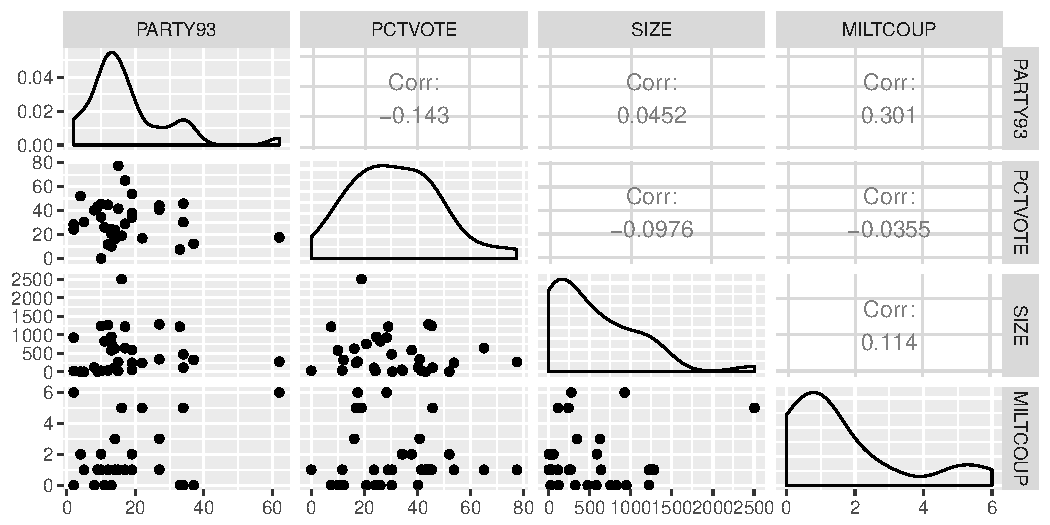
\includegraphics[width=\maxwidth]{figure/pairs-1} 

\end{knitrout}

Response is non-negative
\end{frame}


\begin{frame}{Poisson Distribution}
  \begin{align*}
 Y_i \mid \lambda_i & \sim P(\lambda_i)     \\
p(y_i) & = \frac{\lambda_i^{y_i} e^{-\lambda_i}}{y_i !} \qquad y_i = 0, 1, \ldots,
\qquad \lambda_i > 0
  \end{align*}  \pause

  \begin{itemize}
  \item Used for counts with no upper limit   \pause
  \item $E(Y_i) = V(Y_i) = \lambda_i$  \pause
  \end{itemize}

How to build in covariates into the mean?  \pause
\begin{itemize}
\item $\lambda > 0  \Leftrightarrow \log(\lambda) = \eta \in \bbR$
\item log link
\end{itemize}
\end{frame}


\begin{frame}{Generalized Linear Model}
Canonical Link function for Poisson data is the log link   \pause
\begin{itemize}
\item $\log(\lambda_i) = \eta_i = \beta_0 + X_1 \beta_1 + \ldots X_p \beta_p $ (linear predictor)  \pause
\item $\lambda = \exp( \beta_0 + X_1 \beta_1 + \ldots X_p \beta_p) $  \pause
\item Holding all other $X$'s fixed a 1 unit change in $X_j$  \pause
  \begin{align*}
     \lambda^* & = \exp( \beta_0 + X_1 \beta_1 + \ldots (X_j + 1)\beta_j
     + \ldots X_p \beta_p) \\ \pause
 \lambda^* & = \exp(\beta_j) \exp( \beta_0 + X_1 \beta_1 + \ldots X_j \beta_j
     + \ldots X_p \beta_p) \\  \pause
\lambda^* & = \exp(\beta_j) \lambda \\  \pause
\lambda^*/\lambda & =  \exp(\beta_j)
  \end{align*}
\item $\exp(\beta_j)$ is called a ``relative risk''  (risk relative to
  some baseline)
\end{itemize}
\end{frame}

\begin{frame}[fragile]\frametitle{Output from glm}
\begin{small}
\begin{knitrout}
\definecolor{shadecolor}{rgb}{0.969, 0.969, 0.969}\color{fgcolor}\begin{kframe}
\begin{alltt}
\hlstd{africa.glm} \hlkwb{=} \hlkwd{glm}\hlstd{(MILTCOUP} \hlopt{~} \hlstd{MILITARY} \hlopt{+} \hlstd{POLLIB} \hlopt{+} \hlstd{PARTY93}\hlopt{+}
                   \hlstd{PCTVOTE} \hlopt{+} \hlstd{PCTTURN} \hlopt{+} \hlstd{SIZE}\hlopt{*}\hlstd{POP} \hlopt{+}
                   \hlstd{NUMREGIM}\hlopt{*}\hlstd{NUMELEC,}
                   \hlkwc{family}\hlstd{=poisson,} \hlkwc{data}\hlstd{=africa)}
\hlkwd{round}\hlstd{(}\hlkwd{summary}\hlstd{(africa.glm)}\hlopt{$}\hlstd{coef,} \hlnum{4}\hlstd{)}
\end{alltt}
\begin{verbatim}
##                  Estimate Std. Error z value Pr(>|z|)
## (Intercept)        2.9209     1.3368  2.1850   0.0289
## MILITARY           0.1709     0.0509  3.3575   0.0008
## POLLIB            -0.4654     0.3319 -1.4022   0.1609
## PARTY93            0.0247     0.0109  2.2792   0.0227
## PCTVOTE            0.0613     0.0217  2.8202   0.0048
## PCTTURN           -0.0361     0.0137 -2.6372   0.0084
## SIZE              -0.0018     0.0007 -2.5223   0.0117
## POP               -0.1188     0.0397 -2.9961   0.0027
## NUMREGIM          -0.8662     0.4571 -1.8949   0.0581
## NUMELEC           -0.4859     0.2118 -2.2948   0.0217
## SIZE:POP           0.0001     0.0000  3.0111   0.0026
## NUMREGIM:NUMELEC   0.1810     0.0689  2.6265   0.0086
\end{verbatim}
\end{kframe}
\end{knitrout}
\end{small}
\end{frame}


\begin{frame}[fragile]\frametitle{lack of fit?}

 \begin{itemize}
    \item Under the hypothesis that the model is correct,
    residual deviance   has an asymptotic  $\chi^2_{n - p -1}$ distribution  \pause
    \item Residual deviance is the change in deviance from the model to a saturated model where each observation has its own $\lambda_i$
\item Under the alternative that we have omitted important terms,
  expect to see a large residual deviance
 \pause
\item Compare observed deviance to $\chi^2$ distribution
%\item p-value = $P(\chi^2 _{summary(africa.glm)$df.residual > round{summary(africa.glm)$deviance),2 = 0.996$  \pause
\end{itemize}
\begin{small}
\begin{knitrout}
\definecolor{shadecolor}{rgb}{0.969, 0.969, 0.969}\color{fgcolor}\begin{kframe}
\begin{alltt}
\hlkwd{c}\hlstd{(}\hlkwd{summary}\hlstd{(africa.glm)}\hlopt{$}\hlstd{deviance,} \hlkwd{summary}\hlstd{(africa.glm)}\hlopt{$}\hlstd{df.residual)}
\end{alltt}
\begin{verbatim}
## [1]  7.547369 21.000000
\end{verbatim}
\begin{alltt}
\hlnum{1} \hlopt{-} \hlkwd{pchisq}\hlstd{(}\hlkwd{summary}\hlstd{(africa.glm)}\hlopt{$}\hlstd{deviance,} \hlkwd{summary}\hlstd{(africa.glm)}\hlopt{$}\hlstd{df.residual)}
\end{alltt}
\begin{verbatim}
## [1] 0.9967843
\end{verbatim}
\end{kframe}
\end{knitrout}
\end{small}
So no evidence of lack of fit (overdispersion).
\end{frame}


\begin{frame}[fragile]\frametitle{Diagnostics}
\begin{knitrout}
\definecolor{shadecolor}{rgb}{0.969, 0.969, 0.969}\color{fgcolor}
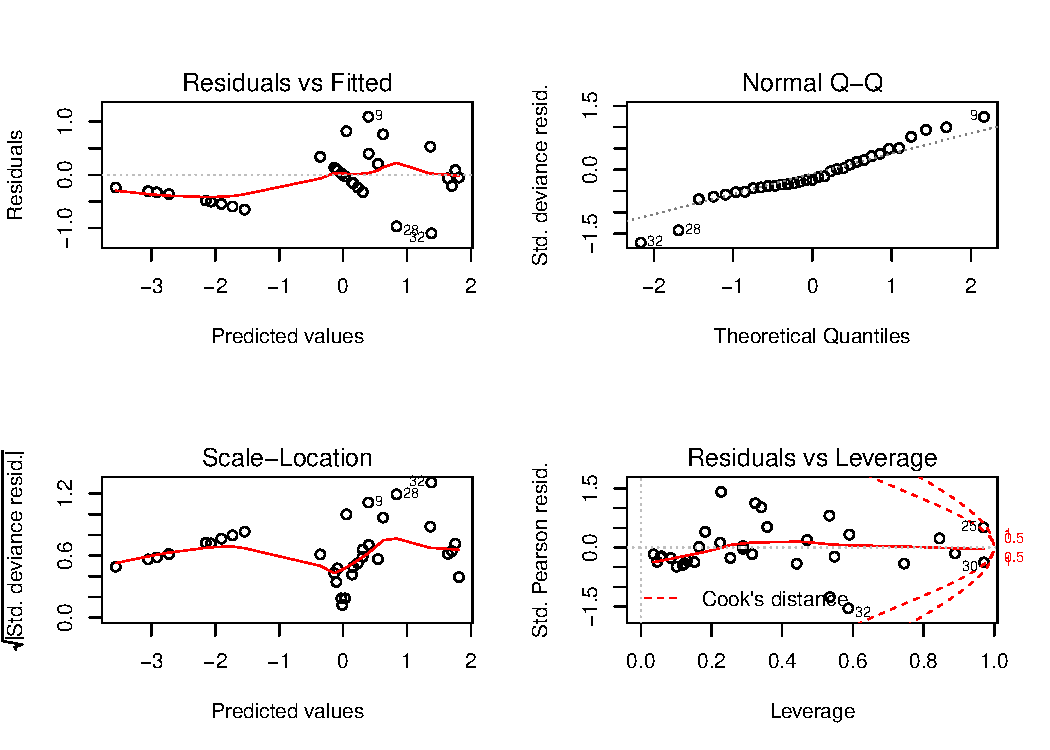
\includegraphics[width=\maxwidth]{figure/diag-1} 

\end{knitrout}

\end{frame}

\begin{frame} {Residuals in GLMS}

\begin{itemize}
\item residuals:  $Y_i - \hat{\lambda}_i$  (observed - fitted)
\item Pearson Goodness of Fit
$$X^2 = \sum_i \frac{(Y_i -  \hat{\lambda}_i)^2} {\hat{\lambda}_i}$$
\item Pearson Residuals:
$$r_i =  \frac{Y_i -  \hat{\lambda}_i}  {\sqrt{ \hat{\lambda}_i } }$$
{\tt residuals.glm(africa.glm, type="pearson")}
\item residual deviance: Change in deviance for Model compared to Saturated model
\begin{align*}
D & = 2 \left\{
\sum_i y_i \log(y_i/\hat{\lambda}_i) - (y_i - \hat{\lambda}_i)
\right\} \\
 &  =  \sum d_i
 \end{align*}
 {\tt residuals.glm(africa.glm, type="deviance")}
\end{itemize}
\end{frame}


\begin{frame}[fragile]{Coefficients}
% latex table generated in R 3.3.2 by xtable 1.8-2 package
% Mon Feb  6 18:53:54 2017
\begin{table}[ht]
\centering
\begin{tabular}{rrrrr}
  \hline
 & Estimate & Std. Error & z value & Pr($>$$|$z$|$) \\ 
  \hline
(Intercept) & 2.92 & 1.34 & 2.18 & 0.03 \\ 
  MILITARY & 0.17 & 0.05 & 3.36 & 0.00 \\ 
  POLLIB & -0.47 & 0.33 & -1.40 & 0.16 \\ 
  PARTY93 & 0.02 & 0.01 & 2.28 & 0.02 \\ 
  PCTVOTE & 0.06 & 0.02 & 2.82 & 0.00 \\ 
  PCTTURN & -0.04 & 0.01 & -2.64 & 0.01 \\ 
  SIZE & -0.00 & 0.00 & -2.52 & 0.01 \\ 
  POP & -0.12 & 0.04 & -3.00 & 0.00 \\ 
  NUMREGIM & -0.87 & 0.46 & -1.89 & 0.06 \\ 
  NUMELEC & -0.49 & 0.21 & -2.29 & 0.02 \\ 
  SIZE:POP & 0.00 & 0.00 & 3.01 & 0.00 \\ 
  NUMREGIM:NUMELEC & 0.18 & 0.07 & 2.63 & 0.01 \\ 
   \hline
\end{tabular}
\end{table}


\end{frame}


\begin{frame}[fragile]{Treat Political Liberties as a Factor?}
\begin{knitrout}
\definecolor{shadecolor}{rgb}{0.969, 0.969, 0.969}\color{fgcolor}\begin{kframe}
\begin{alltt}
\hlstd{africa.glm1} \hlkwb{=} \hlkwd{glm}\hlstd{(MILTCOUP} \hlopt{~} \hlstd{MILITARY} \hlopt{+} \hlkwd{factor}\hlstd{(POLLIB)} \hlopt{+}
                    \hlstd{PARTY93} \hlopt{+} \hlstd{PCTVOTE}\hlopt{+} \hlstd{PCTTURN} \hlopt{+}
                    \hlstd{SIZE}\hlopt{*}\hlstd{POP} \hlopt{+} \hlstd{NUMREGIM}\hlopt{*}\hlstd{NUMELEC,}
                    \hlkwc{family}\hlstd{=poisson,} \hlkwc{data}\hlstd{=africa)}
\hlkwd{anova}\hlstd{(africa.glm, africa.glm1,} \hlkwc{test}\hlstd{=}\hlstr{"Chi"}\hlstd{)}
\end{alltt}
\begin{verbatim}
## Analysis of Deviance Table
## 
## Model 1: MILTCOUP ~ MILITARY + POLLIB + PARTY93 + PCTVOTE + PCTTURN + 
##     SIZE * POP + NUMREGIM * NUMELEC
## Model 2: MILTCOUP ~ MILITARY + factor(POLLIB) + PARTY93 + PCTVOTE + PCTTURN + 
##     SIZE * POP + NUMREGIM * NUMELEC
##   Resid. Df Resid. Dev Df Deviance Pr(>Chi)
## 1        21     7.5474                     
## 2        20     7.1316  1  0.41581    0.519
\end{verbatim}
\end{kframe}
\end{knitrout}

\end{frame}


\begin{frame}[fragile]\frametitle{Interpretation of Coefficients}

  \begin{itemize}
  \item Asymptotic distribution (Frequentist)
$$(\beta_j - \hat{\beta_j})/\SE(\beta_j) \sim N(0,1)$$  \pause
  \item 95\% CI for coefficient of MILITARY:
   $$0.171 \pm 1.96 \cdot 0.051  = (
   0.078, 0.282)$$  \pause
  \item relative risk is $\exp(0.171) = 1.186$  \pause
  \item  95\% CI for relative risk  $e^{CI}$
$$ (\exp(0.078), \exp(0.282))  =
(1.081, 1.325)$$
%$$
  \end{itemize}

Keeping everything else constant, for every additional year of military oligarchy, the risk of a
military coup increases by $8$ to $32$ percent

\end{frame}

\begin{frame}\frametitle{Deviance Goodness of Fit}
\begin{itemize}
\item deviance is -2 log(likelihood) evaluated at the MLE of the parameters in that model
$$ -2 \sum_i (y_i \log(\hat{\lambda}_i)  + \hat{\lambda}_i -
\log( y_i!))$$
\item smaller is better (larger likelihood)
\item null deviance is the deviance under the "Null" model, that is a model with just an intercept or $\lambda_i = \lambda$ and $\hat{\lambda} = \bar{Y}$
\item saturated model deviance is the deviance of a model where each observation has there own unique $\lambda_i$ and the MLE of $\hat{\lambda}_i = y_i$,
\item the change in deviance has a Chi-squared distribution
with degrees of freedom equal to the change in number of parameters in the models.
\end{itemize}
\end{frame}


\begin{frame} \frametitle{Derivation}
the residual deviance is the change in the deviance between the given model and the saturated model. substituting, we have
\begin{align*}
D  = & -2\sum_i\left(y_i \log(\hat{\lambda}_i)  - \hat{\lambda}_i -
\log(y_i!)\right) - \\
&  -2\sum_i\left (y_i \log(y_i)  - y_i -
\log(y_i!)\right) \\
=  & 2 \sum_i\left(y_i (\log(y_i) -  \log(\hat{\lambda}_i))   -( y_i -  \hat{\lambda}_i)) \right) \\
& = 2 \left(y_i (\log(y_i/\hat{\lambda}_i)   - (y_i -  \hat{\lambda}_i)) \right)
& = \sum 2 d_i
\end{align*}
This has a chi squared distibution with $n - (p+1)$ degrees of freedom.
\end{frame}
\end{document}
